\INEchaptercarta{Nacimientos: características escolares de las madres}{}

\cajita{Nacimientos}{La cantidad de nacimientos registrados en el 2014 tuvo una disminución del 0.32\% respecto al año anterior.}{Nacimientos registrados}{República de Guatemala, serie histórica, en datos absolutos}{\ \\[0mm]\begin{tikzpicture}[x=1pt,y=1pt]  % Created by tikzDevice version 0.8.1 on 2015-12-10 16:21:53
% !TEX encoding = UTF-8 Unicode
\definecolor{fillColor}{RGB}{255,255,255}
\path[use as bounding box,fill=fillColor,fill opacity=0.00] (0,0) rectangle (289.08,198.74);
\begin{scope}
\path[clip] (  0.00,  0.00) rectangle (289.08,198.74);

\path[] (  0.00,  0.00) rectangle (289.08,198.74);
\end{scope}
\begin{scope}
\path[clip] (  0.00,  0.00) rectangle (289.08,198.74);

\path[] ( 19.16, 17.78) rectangle (280.54,191.48);

\path[] ( 19.16, 42.22) --
	(280.54, 42.22);

\path[] ( 19.16, 75.31) --
	(280.54, 75.31);

\path[] ( 19.16,108.40) --
	(280.54,108.40);

\path[] ( 19.16,141.49) --
	(280.54,141.49);

\path[] ( 19.16,174.58) --
	(280.54,174.58);

\path[] ( 19.16, 25.67) --
	(280.54, 25.67);

\path[] ( 19.16, 58.76) --
	(280.54, 58.76);

\path[] ( 19.16, 91.85) --
	(280.54, 91.85);

\path[] ( 19.16,124.94) --
	(280.54,124.94);

\path[] ( 19.16,158.03) --
	(280.54,158.03);

\path[] ( 19.16,191.12) --
	(280.54,191.12);

\path[] ( 49.32, 17.78) --
	( 49.32,191.48);

\path[] ( 99.59, 17.78) --
	( 99.59,191.48);

\path[] (149.85, 17.78) --
	(149.85,191.48);

\path[] (200.12, 17.78) --
	(200.12,191.48);

\path[] (250.38, 17.78) --
	(250.38,191.48);
\definecolor{drawColor}{RGB}{0,0,255}

\path[draw=drawColor,line width= 1.7pt,line join=round] ( 49.32,165.91) --
	( 99.59,173.71) --
	(149.85,183.59) --
	(200.12,182.75) --
	(250.38,181.99);
\definecolor{drawColor}{RGB}{0,0,0}

\node[text=drawColor,anchor=base,inner sep=0pt, outer sep=0pt, scale=  1.01] at ( 49.32,154.04) {361,906};

\node[text=drawColor,anchor=base east,inner sep=0pt, outer sep=0pt, scale=  1.01] at ( 93.81,173.71) {373,692};

\node[text=drawColor,anchor=base,inner sep=0pt, outer sep=0pt, scale=  1.01] at (149.85,187.54) {388,613};

\node[text=drawColor,anchor=base west,inner sep=0pt, outer sep=0pt, scale=  1.01] at (200.12,186.70) {387,342};

\node[text=drawColor,anchor=base,inner sep=0pt, outer sep=0pt, scale=  1.01] at (250.38,170.12) {386,195};

\path[draw=drawColor,line width= 0.1pt,line join=round] ( 19.16, 25.67) -- (280.54, 25.67);

\path[] ( 19.16, 17.78) rectangle (280.54,191.48);
\end{scope}
\begin{scope}
\path[clip] (  0.00,  0.00) rectangle (289.08,198.74);

\path[] ( 19.16, 17.78) --
	( 19.16,191.48);
\end{scope}
\begin{scope}
\path[clip] (  0.00,  0.00) rectangle (289.08,198.74);
\definecolor{drawColor}{RGB}{255,255,255}

\node[text=drawColor,text opacity=0.00,anchor=base east,inner sep=0pt, outer sep=0pt, scale=  1.00] at ( 12.05, 21.76) {150000};

\node[text=drawColor,text opacity=0.00,anchor=base east,inner sep=0pt, outer sep=0pt, scale=  1.00] at ( 12.05, 54.85) {200000};

\node[text=drawColor,text opacity=0.00,anchor=base east,inner sep=0pt, outer sep=0pt, scale=  1.00] at ( 12.05, 87.94) {250000};

\node[text=drawColor,text opacity=0.00,anchor=base east,inner sep=0pt, outer sep=0pt, scale=  1.00] at ( 12.05,121.03) {300000};

\node[text=drawColor,text opacity=0.00,anchor=base east,inner sep=0pt, outer sep=0pt, scale=  1.00] at ( 12.05,154.12) {350000};

\node[text=drawColor,text opacity=0.00,anchor=base east,inner sep=0pt, outer sep=0pt, scale=  1.00] at ( 12.05,187.21) {400000};
\end{scope}
\begin{scope}
\path[clip] (  0.00,  0.00) rectangle (289.08,198.74);

\path[] ( 14.89, 25.67) --
	( 19.16, 25.67);

\path[] ( 14.89, 58.76) --
	( 19.16, 58.76);

\path[] ( 14.89, 91.85) --
	( 19.16, 91.85);

\path[] ( 14.89,124.94) --
	( 19.16,124.94);

\path[] ( 14.89,158.03) --
	( 19.16,158.03);

\path[] ( 14.89,191.12) --
	( 19.16,191.12);
\end{scope}
\begin{scope}
\path[clip] (  0.00,  0.00) rectangle (289.08,198.74);

\path[] ( 19.16, 17.78) --
	(280.54, 17.78);
\end{scope}
\begin{scope}
\path[clip] (  0.00,  0.00) rectangle (289.08,198.74);

\path[] ( 49.32, 13.51) --
	( 49.32, 17.78);

\path[] ( 99.59, 13.51) --
	( 99.59, 17.78);

\path[] (149.85, 13.51) --
	(149.85, 17.78);

\path[] (200.12, 13.51) --
	(200.12, 17.78);

\path[] (250.38, 13.51) --
	(250.38, 17.78);
\end{scope}
\begin{scope}
\path[clip] (  0.00,  0.00) rectangle (289.08,198.74);
\definecolor{drawColor}{RGB}{0,0,0}

\node[text=drawColor,anchor=base,inner sep=0pt, outer sep=0pt, scale=  1.00] at ( 49.32,  2.85) {2010};

\node[text=drawColor,anchor=base,inner sep=0pt, outer sep=0pt, scale=  1.00] at ( 99.59,  2.85) {2011};

\node[text=drawColor,anchor=base,inner sep=0pt, outer sep=0pt, scale=  1.00] at (149.85,  2.85) {2012};

\node[text=drawColor,anchor=base,inner sep=0pt, outer sep=0pt, scale=  1.00] at (200.12,  2.85) {2013};

\node[text=drawColor,anchor=base,inner sep=0pt, outer sep=0pt, scale=  1.00] at (250.38,  2.85) {2014};
\end{scope}
  \end{tikzpicture}}{Instituto Nacional de Estadística, de las Estadísticas Vitales 2014}

\cajita{Escolaridad de la madre}{De los nacimientos ocurridos en el 2014, el 37.5\% fueron en madres con escolaridad en el nivel primario; el 31.2\% en mujeres sin ningún nivel de escolaridad.}{Distribución de los nacimientos según escolaridad de la madre }{República de Guatemala, 2014, en porcentaje}{\ \\[0mm]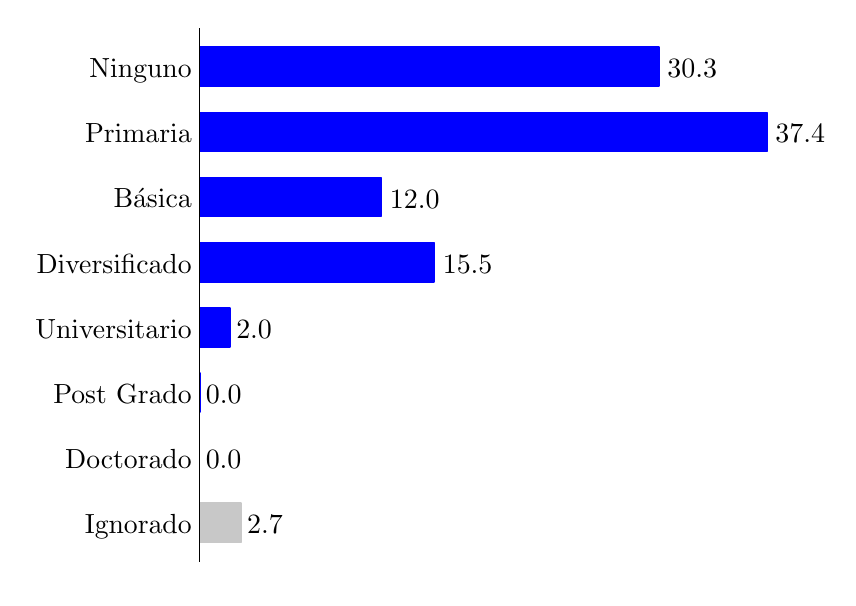
\begin{tikzpicture}[x=1pt,y=1pt]  % Created by tikzDevice version 0.8.1 on 2015-12-10 16:21:53
% !TEX encoding = UTF-8 Unicode
\definecolor{fillColor}{RGB}{255,255,255}
\path[use as bounding box,fill=fillColor,fill opacity=0.00] (0,0) rectangle (289.08,198.74);
\begin{scope}
\path[clip] (  0.00,  0.00) rectangle (289.08,198.74);

\path[] (  0.00,  0.00) rectangle (289.08,198.74);
\end{scope}
\begin{scope}
\path[clip] (  0.00,  0.00) rectangle (289.08,198.74);

\path[] ( 62.12,  5.69) rectangle (267.09,198.74);

\path[] ( 62.12, 19.82) --
	(267.09, 19.82);

\path[] ( 62.12, 43.36) --
	(267.09, 43.36);

\path[] ( 62.12, 66.90) --
	(267.09, 66.90);

\path[] ( 62.12, 90.45) --
	(267.09, 90.45);

\path[] ( 62.12,113.99) --
	(267.09,113.99);

\path[] ( 62.12,137.53) --
	(267.09,137.53);

\path[] ( 62.12,161.07) --
	(267.09,161.07);

\path[] ( 62.12,184.62) --
	(267.09,184.62);
\definecolor{drawColor}{RGB}{200,200,200}
\definecolor{fillColor}{RGB}{200,200,200}

\path[draw=drawColor,line width= 0.6pt,line join=round,fill=fillColor] ( 62.12, 12.75) rectangle ( 77.04, 26.88);
\definecolor{drawColor}{RGB}{0,0,255}
\definecolor{fillColor}{RGB}{0,0,255}

\path[draw=drawColor,line width= 0.6pt,line join=round,fill=fillColor] ( 62.12, 36.30) rectangle ( 62.12, 50.42);

\path[draw=drawColor,line width= 0.6pt,line join=round,fill=fillColor] ( 62.12, 59.84) rectangle ( 62.20, 73.97);

\path[draw=drawColor,line width= 0.6pt,line join=round,fill=fillColor] ( 62.12, 83.38) rectangle ( 73.14, 97.51);

\path[draw=drawColor,line width= 0.6pt,line join=round,fill=fillColor] ( 62.12,106.93) rectangle (146.89,121.05);

\path[draw=drawColor,line width= 0.6pt,line join=round,fill=fillColor] ( 62.12,130.47) rectangle (127.76,144.59);

\path[draw=drawColor,line width= 0.6pt,line join=round,fill=fillColor] ( 62.12,154.01) rectangle (267.09,168.14);

\path[draw=drawColor,line width= 0.6pt,line join=round,fill=fillColor] ( 62.12,177.55) rectangle (228.02,191.68);
\definecolor{drawColor}{RGB}{0,0,0}

\path[draw=drawColor,line width= 0.1pt,line join=round] ( 62.12,  5.69) -- ( 62.12,198.74);

\node[text=drawColor,anchor=base west,inner sep=0pt, outer sep=0pt, scale=  1.01] at ( 79.27, 15.86) {2.7};

\node[text=drawColor,anchor=base west,inner sep=0pt, outer sep=0pt, scale=  1.01] at ( 64.35, 39.40) {0.0};

\node[text=drawColor,anchor=base west,inner sep=0pt, outer sep=0pt, scale=  1.01] at ( 64.43, 62.95) {0.0};

\node[text=drawColor,anchor=base west,inner sep=0pt, outer sep=0pt, scale=  1.01] at ( 75.37, 86.49) {2.0};

\node[text=drawColor,anchor=base west,inner sep=0pt, outer sep=0pt, scale=  1.01] at (150.00,110.03) {15.5};

\node[text=drawColor,anchor=base west,inner sep=0pt, outer sep=0pt, scale=  1.01] at (130.88,133.57) {12.0};

\node[text=drawColor,anchor=base west,inner sep=0pt, outer sep=0pt, scale=  1.01] at (270.20,157.12) {37.4};

\node[text=drawColor,anchor=base west,inner sep=0pt, outer sep=0pt, scale=  1.01] at (231.14,180.66) {30.3};

\path[] ( 62.12,  5.69) rectangle (267.09,198.74);
\end{scope}
\begin{scope}
\path[clip] (  0.00,  0.00) rectangle (289.08,198.74);

\path[] ( 62.12,  5.69) --
	( 62.12,198.74);
\end{scope}
\begin{scope}
\path[clip] (  0.00,  0.00) rectangle (289.08,198.74);
\definecolor{drawColor}{RGB}{0,0,0}

\node[text=drawColor,anchor=base east,inner sep=0pt, outer sep=0pt, scale=  1.00] at ( 59.27, 15.91) {Ignorado};

\node[text=drawColor,anchor=base east,inner sep=0pt, outer sep=0pt, scale=  1.00] at ( 59.27, 39.45) {Doctorado};

\node[text=drawColor,anchor=base east,inner sep=0pt, outer sep=0pt, scale=  1.00] at ( 59.27, 62.99) {Post Grado};

\node[text=drawColor,anchor=base east,inner sep=0pt, outer sep=0pt, scale=  1.00] at ( 59.27, 86.54) {Universitario};

\node[text=drawColor,anchor=base east,inner sep=0pt, outer sep=0pt, scale=  1.00] at ( 59.27,110.08) {Diversificado};

\node[text=drawColor,anchor=base east,inner sep=0pt, outer sep=0pt, scale=  1.00] at ( 59.27,133.62) {Básica};

\node[text=drawColor,anchor=base east,inner sep=0pt, outer sep=0pt, scale=  1.00] at ( 59.27,157.17) {Primaria};

\node[text=drawColor,anchor=base east,inner sep=0pt, outer sep=0pt, scale=  1.00] at ( 59.27,180.71) {Ninguno};
\end{scope}
\begin{scope}
\path[clip] (  0.00,  0.00) rectangle (289.08,198.74);

\path[] ( 59.27, 19.82) --
	( 63.54, 19.82);

\path[] ( 59.27, 43.36) --
	( 63.54, 43.36);

\path[] ( 59.27, 66.90) --
	( 63.54, 66.90);

\path[] ( 59.27, 90.45) --
	( 63.54, 90.45);

\path[] ( 59.27,113.99) --
	( 63.54,113.99);

\path[] ( 59.27,137.53) --
	( 63.54,137.53);

\path[] ( 59.27,161.07) --
	( 63.54,161.07);

\path[] ( 59.27,184.62) --
	( 63.54,184.62);
\end{scope}
\begin{scope}
\path[clip] (  0.00,  0.00) rectangle (289.08,198.74);

\path[] ( 62.12,  5.69) --
	(267.09,  5.69);
\end{scope}
  \end{tikzpicture}}{Instituto Nacional de Estadística, de las Estadísticas Vitales 2014}

\cajita{Madres sin escolaridad}{La proporción de nacimientos en madres sin escolaridad ha tenido una tendencia descendente, de 37.8\% a 31.2\%, en el período 2010-2014.}{Proporción de nacimientos en madres sin escolaridad}{República de Guatemala, serie histórica, en porcentaje}{\ \\[0mm]\begin{tikzpicture}[x=1pt,y=1pt]  % Created by tikzDevice version 0.8.1 on 2015-12-10 16:21:53
% !TEX encoding = UTF-8 Unicode
\definecolor{fillColor}{RGB}{255,255,255}
\path[use as bounding box,fill=fillColor,fill opacity=0.00] (0,0) rectangle (289.08,198.74);
\begin{scope}
\path[clip] (  0.00,  0.00) rectangle (289.08,198.74);

\path[] (  0.00,  0.00) rectangle (289.08,198.74);
\end{scope}
\begin{scope}
\path[clip] (  0.00,  0.00) rectangle (289.08,198.74);

\path[] (  1.64, 17.78) rectangle (280.54,191.48);

\path[] (  1.64, 46.56) --
	(280.54, 46.56);

\path[] (  1.64, 88.34) --
	(280.54, 88.34);

\path[] (  1.64,130.11) --
	(280.54,130.11);

\path[] (  1.64,171.89) --
	(280.54,171.89);

\path[] (  1.64, 25.67) --
	(280.54, 25.67);

\path[] (  1.64, 67.45) --
	(280.54, 67.45);

\path[] (  1.64,109.22) --
	(280.54,109.22);

\path[] (  1.64,151.00) --
	(280.54,151.00);

\path[] ( 33.83, 17.78) --
	( 33.83,191.48);

\path[] ( 87.46, 17.78) --
	( 87.46,191.48);

\path[] (141.09, 17.78) --
	(141.09,191.48);

\path[] (194.73, 17.78) --
	(194.73,191.48);

\path[] (248.36, 17.78) --
	(248.36,191.48);
\definecolor{drawColor}{RGB}{0,0,255}

\path[draw=drawColor,line width= 1.7pt,line join=round] ( 33.83,183.59) --
	( 87.46,177.32) --
	(141.09,163.53) --
	(194.73,156.01) --
	(248.36,152.31);
\definecolor{drawColor}{RGB}{0,0,0}

\node[text=drawColor,anchor=base,inner sep=0pt, outer sep=0pt, scale=  1.01] at ( 33.83,187.54) {37.8};

\node[text=drawColor,anchor=base west,inner sep=0pt, outer sep=0pt, scale=  1.01] at ( 87.46,181.28) {36.3};

\node[text=drawColor,anchor=base west,inner sep=0pt, outer sep=0pt, scale=  1.01] at (141.09,167.49) {33.0};

\node[text=drawColor,anchor=base west,inner sep=0pt, outer sep=0pt, scale=  1.01] at (194.73,159.97) {31.2};

\node[text=drawColor,anchor=base,inner sep=0pt, outer sep=0pt, scale=  1.01] at (248.36,140.44) {30.3};

\path[draw=drawColor,line width= 0.1pt,line join=round] (  1.64, 25.67) -- (280.54, 25.67);

\path[] (  1.64, 17.78) rectangle (280.54,191.48);
\end{scope}
\begin{scope}
\path[clip] (  0.00,  0.00) rectangle (289.08,198.74);

\path[] (  1.64, 17.78) --
	(  1.64,191.48);
\end{scope}
\begin{scope}
\path[clip] (  0.00,  0.00) rectangle (289.08,198.74);

\path[] (  0.00, 25.67) --
	(  1.64, 25.67);

\path[] (  0.00, 67.45) --
	(  1.64, 67.45);

\path[] (  0.00,109.22) --
	(  1.64,109.22);

\path[] (  0.00,151.00) --
	(  1.64,151.00);
\end{scope}
\begin{scope}
\path[clip] (  0.00,  0.00) rectangle (289.08,198.74);

\path[] (  1.64, 17.78) --
	(280.54, 17.78);
\end{scope}
\begin{scope}
\path[clip] (  0.00,  0.00) rectangle (289.08,198.74);

\path[] ( 33.83, 13.51) --
	( 33.83, 17.78);

\path[] ( 87.46, 13.51) --
	( 87.46, 17.78);

\path[] (141.09, 13.51) --
	(141.09, 17.78);

\path[] (194.73, 13.51) --
	(194.73, 17.78);

\path[] (248.36, 13.51) --
	(248.36, 17.78);
\end{scope}
\begin{scope}
\path[clip] (  0.00,  0.00) rectangle (289.08,198.74);
\definecolor{drawColor}{RGB}{0,0,0}

\node[text=drawColor,anchor=base,inner sep=0pt, outer sep=0pt, scale=  1.00] at ( 33.83,  2.85) {2010};

\node[text=drawColor,anchor=base,inner sep=0pt, outer sep=0pt, scale=  1.00] at ( 87.46,  2.85) {2011};

\node[text=drawColor,anchor=base,inner sep=0pt, outer sep=0pt, scale=  1.00] at (141.09,  2.85) {2012};

\node[text=drawColor,anchor=base,inner sep=0pt, outer sep=0pt, scale=  1.00] at (194.73,  2.85) {2013};

\node[text=drawColor,anchor=base,inner sep=0pt, outer sep=0pt, scale=  1.00] at (248.36,  2.85) {2014};
\end{scope}
  \end{tikzpicture}}{Instituto Nacional de Estadística, de las Estadísticas Vitales 2014}	

\cajita{Madres sin escolaridad por etnia}{La proporción de nacimientos en madres sin escolaridad según su grupo étnico es del 45\% en las madres indígenas, no tenían ningún nivel de escolaridad. De las madres no indígenas era el 16.5\%.}{Proporción de nacimientos en madres sin escolaridad}{República de Guatemala, serie histórica, en porcentaje}{\ \\[0mm]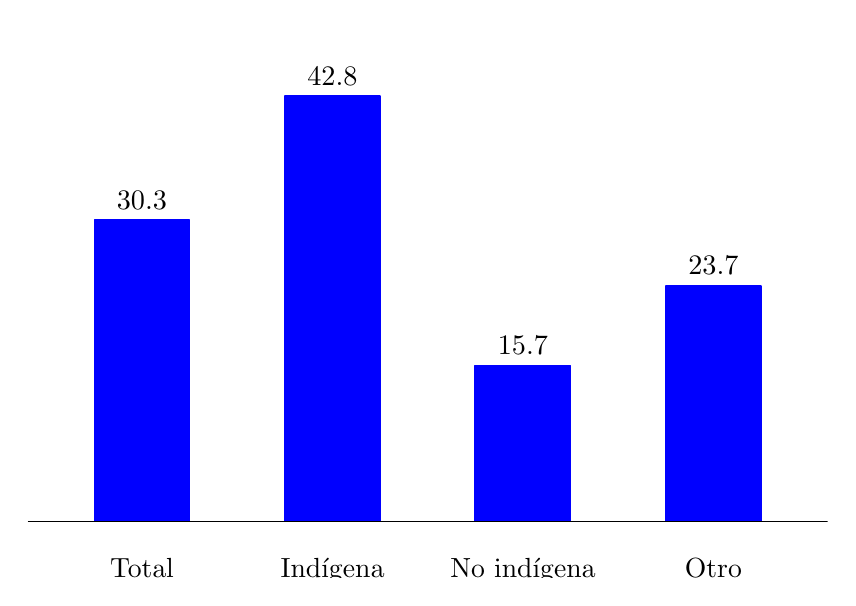
\begin{tikzpicture}[x=1pt,y=1pt]  % Created by tikzDevice version 0.10.1 on 2016-02-29 14:39:15
% !TEX encoding = UTF-8 Unicode
\definecolor{fillColor}{RGB}{255,255,255}
\path[use as bounding box,fill=fillColor,fill opacity=0.00] (0,0) rectangle (289.08,198.74);
\begin{scope}
\path[clip] (  0.00,  0.00) rectangle (289.08,198.74);

\path[] (  0.00,  0.00) rectangle (289.08,198.74);
\end{scope}
\begin{scope}
\path[clip] (  0.00,  0.00) rectangle (289.08,198.74);

\path[] (  0.00, 12.77) rectangle (289.08,181.67);

\path[] ( 41.30, 12.77) --
	( 41.30,181.67);

\path[] (110.13, 12.77) --
	(110.13,181.67);

\path[] (178.95, 12.77) --
	(178.95,181.67);

\path[] (247.78, 12.77) --
	(247.78,181.67);
\definecolor{drawColor}{RGB}{0,0,255}
\definecolor{fillColor}{RGB}{0,0,255}

\path[draw=drawColor,line width= 0.6pt,line join=round,fill=fillColor] ( 24.09, 20.44) rectangle ( 58.50,129.14);

\path[draw=drawColor,line width= 0.6pt,line join=round,fill=fillColor] ( 92.92, 20.44) rectangle (127.33,173.99);

\path[draw=drawColor,line width= 0.6pt,line join=round,fill=fillColor] (161.75, 20.44) rectangle (196.16, 76.65);

\path[draw=drawColor,line width= 0.6pt,line join=round,fill=fillColor] (230.58, 20.44) rectangle (264.99,105.47);
\definecolor{drawColor}{RGB}{0,0,0}

\path[draw=drawColor,line width= 0.1pt,line join=round] (  0.00, 20.44) -- (289.08, 20.44);

\node[text=drawColor,anchor=base,inner sep=0pt, outer sep=0pt, scale=  1.02] at ( 41.30,133.11) {30.3};

\node[text=drawColor,anchor=base,inner sep=0pt, outer sep=0pt, scale=  1.02] at (110.13,177.96) {42.8};

\node[text=drawColor,anchor=base,inner sep=0pt, outer sep=0pt, scale=  1.02] at (178.95, 80.62) {15.7};

\node[text=drawColor,anchor=base,inner sep=0pt, outer sep=0pt, scale=  1.02] at (247.78,109.44) {23.7};

\path[] (  0.00, 12.77) rectangle (289.08,181.67);
\end{scope}
\begin{scope}
\path[clip] (  0.00,  0.00) rectangle (289.08,198.74);

\path[] (  0.00, 12.77) --
	(289.08, 12.77);
\end{scope}
\begin{scope}
\path[clip] (  0.00,  0.00) rectangle (289.08,198.74);

\path[] ( 41.30, 10.02) --
	( 41.30, 12.77);

\path[] (110.13, 10.02) --
	(110.13, 12.77);

\path[] (178.95, 10.02) --
	(178.95, 12.77);

\path[] (247.78, 10.02) --
	(247.78, 12.77);
\end{scope}
\begin{scope}
\path[clip] (  0.00,  0.00) rectangle (289.08,198.74);
\definecolor{drawColor}{RGB}{0,0,0}

\node[text=drawColor,anchor=base,inner sep=0pt, outer sep=0pt, scale=  1.00] at ( 41.30, -0.00) {Total};

\node[text=drawColor,anchor=base,inner sep=0pt, outer sep=0pt, scale=  1.00] at (110.13, -0.00) {Indígena};

\node[text=drawColor,anchor=base,inner sep=0pt, outer sep=0pt, scale=  1.00] at (178.95, -0.00) {No indígena};

\node[text=drawColor,anchor=base,inner sep=0pt, outer sep=0pt, scale=  1.00] at (247.78, -0.00) {Otro};
\end{scope}
  \end{tikzpicture}}{Instituto Nacional de Estadística, de las Estadísticas Vitales 2014}

\cajota{Madres sin escolaridad en los departamentos}{Los departamentos que reportan un mayor porcentaje de nacimientos en madres sin escolaridad son de la región II: Alta Verapaz y Baja Verapaz; de la región VI:  Totonicapán y Sololá; de la región VII: Quiché; y de la región IV: Zacapa.
	
	 Los departamentos con menor porcentaje fueron Guatemala, El Progreso, Chimaltenango, Sacatepéquez, Escuintla y Santa Rosa.}{Proporción de nacimientos en madres sin escolaridad }{Departamental, 2014, en porcentaje}{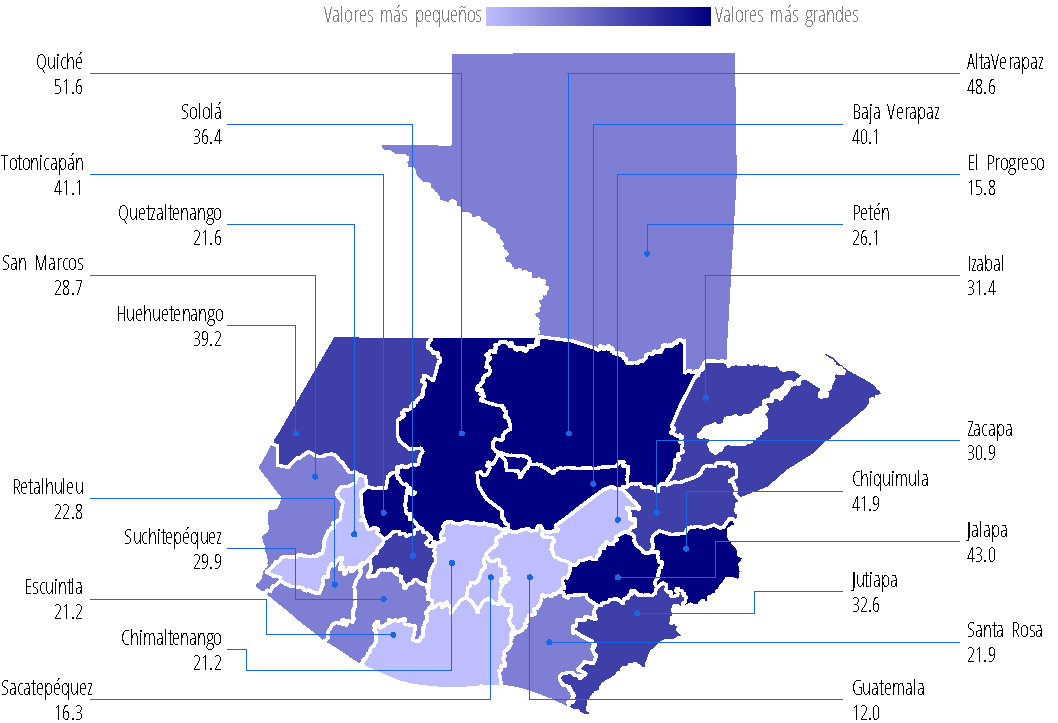
\includegraphics[width=52\cuadri]{graficas/vitales/1_5.pdf}}{Instituto Nacional de Estadística, de las Estadísticas Vitales 2014}

\cajita{Promedio de hijos}{Las madres que tuvieron un nacimiento en el 2014, aquellas sin ningún nivel de escolaridad tenían en promedio 3.7 hijos y las madres con nivel de posgrado, 1.6 hijos.}{Promedio de hijos por madre al momento del nuevo nacimiento, según su escolaridad}{República de Guatemala, 2014, en porcentaje}{\ \\[0mm]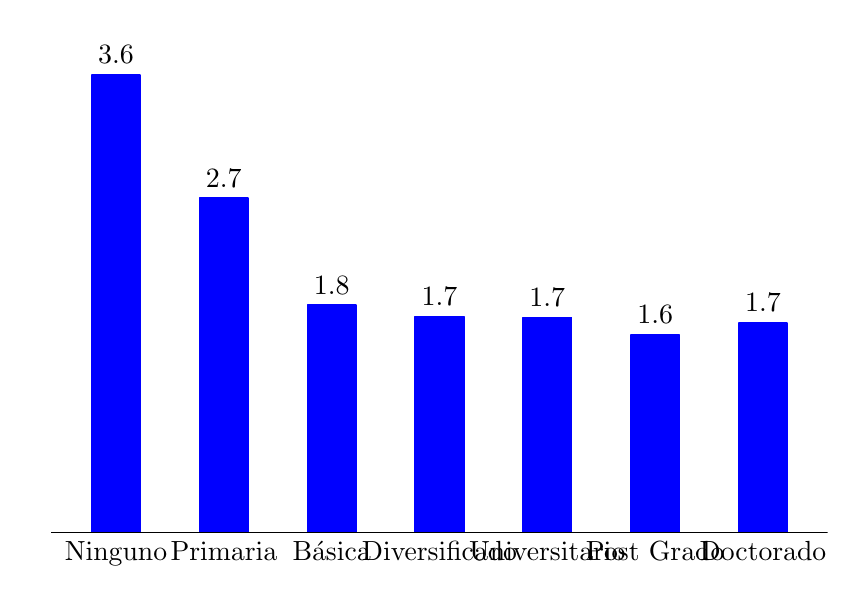
\begin{tikzpicture}[x=1pt,y=1pt]  % Created by tikzDevice version 0.8.1 on 2015-12-10 16:21:53
% !TEX encoding = UTF-8 Unicode
\definecolor{fillColor}{RGB}{255,255,255}
\path[use as bounding box,fill=fillColor,fill opacity=0.00] (0,0) rectangle (289.08,198.74);
\begin{scope}
\path[clip] (  0.00,  0.00) rectangle (289.08,198.74);

\path[] (  0.00,  0.00) rectangle (289.08,198.74);
\end{scope}
\begin{scope}
\path[clip] (  0.00,  0.00) rectangle (289.08,198.74);

\path[] (  8.54, 16.35) rectangle (289.08,181.67);

\path[] ( 31.91, 16.35) --
	( 31.91,181.67);

\path[] ( 70.88, 16.35) --
	( 70.88,181.67);

\path[] (109.84, 16.35) --
	(109.84,181.67);

\path[] (148.81, 16.35) --
	(148.81,181.67);

\path[] (187.77, 16.35) --
	(187.77,181.67);

\path[] (226.74, 16.35) --
	(226.74,181.67);

\path[] (265.70, 16.35) --
	(265.70,181.67);
\definecolor{drawColor}{RGB}{0,0,255}
\definecolor{fillColor}{RGB}{0,0,255}

\path[draw=drawColor,line width= 0.6pt,line join=round,fill=fillColor] ( 23.15, 16.35) rectangle ( 40.68,181.67);

\path[draw=drawColor,line width= 0.6pt,line join=round,fill=fillColor] ( 62.11, 16.35) rectangle ( 79.65,137.08);

\path[draw=drawColor,line width= 0.6pt,line join=round,fill=fillColor] (101.08, 16.35) rectangle (118.61, 98.53);

\path[draw=drawColor,line width= 0.6pt,line join=round,fill=fillColor] (140.04, 16.35) rectangle (157.57, 94.34);

\path[draw=drawColor,line width= 0.6pt,line join=round,fill=fillColor] (179.01, 16.35) rectangle (196.54, 94.07);

\path[draw=drawColor,line width= 0.6pt,line join=round,fill=fillColor] (217.97, 16.35) rectangle (235.50, 87.76);

\path[draw=drawColor,line width= 0.6pt,line join=round,fill=fillColor] (256.93, 16.35) rectangle (274.47, 92.09);
\definecolor{drawColor}{RGB}{0,0,0}

\path[draw=drawColor,line width= 0.1pt,line join=round] (  8.54, 16.35) -- (289.08, 16.35);

\node[text=drawColor,anchor=base,inner sep=0pt, outer sep=0pt, scale=  1.01] at ( 31.91,185.63) {3.6};

\node[text=drawColor,anchor=base,inner sep=0pt, outer sep=0pt, scale=  1.01] at ( 70.88,141.03) {2.7};

\node[text=drawColor,anchor=base,inner sep=0pt, outer sep=0pt, scale=  1.01] at (109.84,102.49) {1.8};

\node[text=drawColor,anchor=base,inner sep=0pt, outer sep=0pt, scale=  1.01] at (148.81, 98.29) {1.7};

\node[text=drawColor,anchor=base,inner sep=0pt, outer sep=0pt, scale=  1.01] at (187.77, 98.02) {1.7};

\node[text=drawColor,anchor=base,inner sep=0pt, outer sep=0pt, scale=  1.01] at (226.74, 91.72) {1.6};

\node[text=drawColor,anchor=base,inner sep=0pt, outer sep=0pt, scale=  1.01] at (265.70, 96.05) {1.7};

\path[] (  8.54, 16.35) rectangle (289.08,181.67);
\end{scope}
\begin{scope}
\path[clip] (  0.00,  0.00) rectangle (289.08,198.74);

\path[] (  8.54, 16.35) --
	(  8.54,181.67);
\end{scope}
\begin{scope}
\path[clip] (  0.00,  0.00) rectangle (289.08,198.74);

\path[] (  8.54, 16.35) --
	(289.08, 16.35);
\end{scope}
\begin{scope}
\path[clip] (  0.00,  0.00) rectangle (289.08,198.74);

\path[] ( 31.91, 12.08) --
	( 31.91, 16.35);

\path[] ( 70.88, 12.08) --
	( 70.88, 16.35);

\path[] (109.84, 12.08) --
	(109.84, 16.35);

\path[] (148.81, 12.08) --
	(148.81, 16.35);

\path[] (187.77, 12.08) --
	(187.77, 16.35);

\path[] (226.74, 12.08) --
	(226.74, 16.35);

\path[] (265.70, 12.08) --
	(265.70, 16.35);
\end{scope}
\begin{scope}
\path[clip] (  0.00,  0.00) rectangle (289.08,198.74);
\definecolor{drawColor}{RGB}{0,0,0}

\node[text=drawColor,anchor=base,inner sep=0pt, outer sep=0pt, scale=  1.00] at ( 31.91,  6.04) {Ninguno};

\node[text=drawColor,anchor=base,inner sep=0pt, outer sep=0pt, scale=  1.00] at ( 70.88,  6.04) {Primaria};

\node[text=drawColor,anchor=base,inner sep=0pt, outer sep=0pt, scale=  1.00] at (109.84,  6.04) {Básica};

\node[text=drawColor,anchor=base,inner sep=0pt, outer sep=0pt, scale=  1.00] at (148.81,  6.04) {Diversificado};

\node[text=drawColor,anchor=base,inner sep=0pt, outer sep=0pt, scale=  1.00] at (187.77,  6.04) {Universitario};

\node[text=drawColor,anchor=base,inner sep=0pt, outer sep=0pt, scale=  1.00] at (226.74,  6.04) {Post Grado};

\node[text=drawColor,anchor=base,inner sep=0pt, outer sep=0pt, scale=  1.00] at (265.70,  6.04) {Doctorado};
\end{scope}
  \end{tikzpicture}}{Instituto Nacional de Estadística, de las Estadísticas Vitales 2014}

\cajita{Promedio de hijos de madres sin escolaridad}{Según los nacimientos reportados cada año, las madres sin ningún nivel de educación han tenido, al momento del nuevo nacimiento, un promedio de 3.7 hijos.}{Promedio de hijos por madre sin educación,\\ al momento del nuevo nacimiento}{República de Guatemala, serie histórica, en porcentaje}{\ \\[0mm]\begin{tikzpicture}[x=1pt,y=1pt]  % Created by tikzDevice version 0.10.1 on 2016-02-29 14:40:32
% !TEX encoding = UTF-8 Unicode
\definecolor{fillColor}{RGB}{255,255,255}
\path[use as bounding box,fill=fillColor,fill opacity=0.00] (0,0) rectangle (289.08,198.74);
\begin{scope}
\path[clip] (  0.00,  0.00) rectangle (289.08,198.74);

\path[] (  0.00,  0.00) rectangle (289.08,198.74);
\end{scope}
\begin{scope}
\path[clip] (  0.00,  0.00) rectangle (289.08,198.74);

\path[] ( -4.90, 15.61) rectangle (280.54,191.48);

\path[] (  0.00, 52.34) --
	(280.54, 52.34);

\path[] (  0.00,109.79) --
	(280.54,109.79);

\path[] (  0.00,167.25) --
	(280.54,167.25);

\path[] (  0.00, 23.61) --
	(280.54, 23.61);

\path[] (  0.00, 81.06) --
	(280.54, 81.06);

\path[] (  0.00,138.52) --
	(280.54,138.52);

\path[] ( 28.04, 15.61) --
	( 28.04,191.48);

\path[] ( 82.93, 15.61) --
	( 82.93,191.48);

\path[] (137.82, 15.61) --
	(137.82,191.48);

\path[] (192.72, 15.61) --
	(192.72,191.48);

\path[] (247.61, 15.61) --
	(247.61,191.48);
\definecolor{drawColor}{RGB}{0,0,255}

\path[draw=drawColor,line width= 1.7pt,line join=round] ( 28.04,182.08) --
	( 82.93,179.87) --
	(137.82,183.49) --
	(192.72,178.74) --
	(247.61,175.17);
\definecolor{drawColor}{RGB}{0,0,0}

\node[text=drawColor,anchor=base,inner sep=0pt, outer sep=0pt, scale=  1.02] at ( 28.04,186.05) {3.8};

\node[text=drawColor,anchor=base,inner sep=0pt, outer sep=0pt, scale=  1.02] at ( 82.93,167.95) {3.7};

\node[text=drawColor,anchor=base,inner sep=0pt, outer sep=0pt, scale=  1.02] at (137.82,187.46) {3.8};

\node[text=drawColor,anchor=base west,inner sep=0pt, outer sep=0pt, scale=  1.02] at (192.72,182.71) {3.7};

\node[text=drawColor,anchor=base,inner sep=0pt, outer sep=0pt, scale=  1.02] at (247.61,163.26) {3.6};

\path[draw=drawColor,line width= 0.1pt,line join=round] (  0.00, 23.61) -- (280.54, 23.61);

\path[] ( -4.90, 15.61) rectangle (280.54,191.48);
\end{scope}
\begin{scope}
\path[clip] (  0.00,  0.00) rectangle (289.08,198.74);

\path[] (  0.00, 15.61) --
	(280.54, 15.61);
\end{scope}
\begin{scope}
\path[clip] (  0.00,  0.00) rectangle (289.08,198.74);

\path[] ( 28.04, 12.86) --
	( 28.04, 15.61);

\path[] ( 82.93, 12.86) --
	( 82.93, 15.61);

\path[] (137.82, 12.86) --
	(137.82, 15.61);

\path[] (192.72, 12.86) --
	(192.72, 15.61);

\path[] (247.61, 12.86) --
	(247.61, 15.61);
\end{scope}
\begin{scope}
\path[clip] (  0.00,  0.00) rectangle (289.08,198.74);
\definecolor{drawColor}{RGB}{0,0,0}

\node[text=drawColor,anchor=base,inner sep=0pt, outer sep=0pt, scale=  1.00] at ( 28.04,  2.85) {2010};

\node[text=drawColor,anchor=base,inner sep=0pt, outer sep=0pt, scale=  1.00] at ( 82.93,  2.85) {2011};

\node[text=drawColor,anchor=base,inner sep=0pt, outer sep=0pt, scale=  1.00] at (137.82,  2.85) {2012};

\node[text=drawColor,anchor=base,inner sep=0pt, outer sep=0pt, scale=  1.00] at (192.72,  2.85) {2013};

\node[text=drawColor,anchor=base,inner sep=0pt, outer sep=0pt, scale=  1.00] at (247.61,  2.85) {2014};
\end{scope}
  \end{tikzpicture}}{Instituto Nacional de Estadística, de las Estadísticas Vitales 2014}


\cajota{Promedio de hijos de madres sin escolaridad en los departamentos}{Según los nacimientos reportados en el 2014, las madres sin ningún nivel de escolaridad, tenían en promedio 3.7 hijos.
	
	 Los departamentos con el mayor número de hijos, en promedio, fueron Quiché y Sololá.}{Promedio de hijos por madre sin educación, al momento del nuevo nacimiento}{Departamental, 2014, en porcentaje}{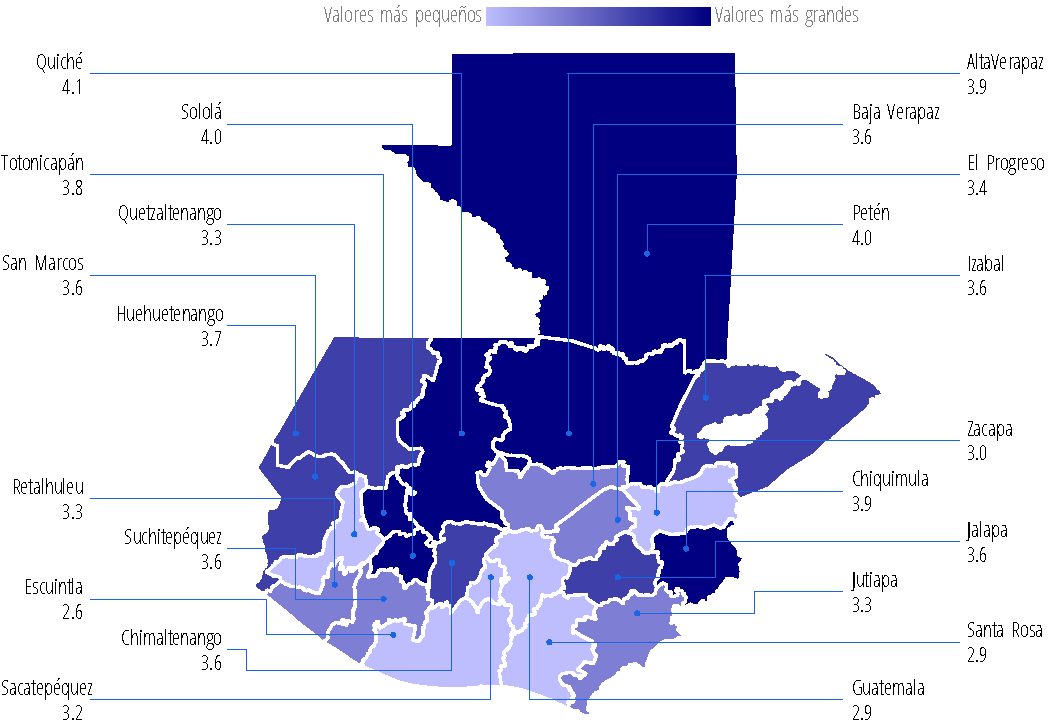
\includegraphics[width=52\cuadri]{graficas/vitales/1_8.pdf}}{Instituto Nacional de Estadística, de las Estadísticas Vitales 2014}

\cajita{Madres que recibieron atención médica}{Los nacimientos ocurridos en el 2014, el 98.5\% de las madres con educación superior recibió asistencia médica, por otro lado, solo el 42.6\% de las madres sin educación tuvo este tipo de atención médica.}{Proporción de nacimientos que recibieron atención médica según nivel de escolaridad de la madre}{República de Guatemala, 2014, en porcentaje}{\ \\[0mm]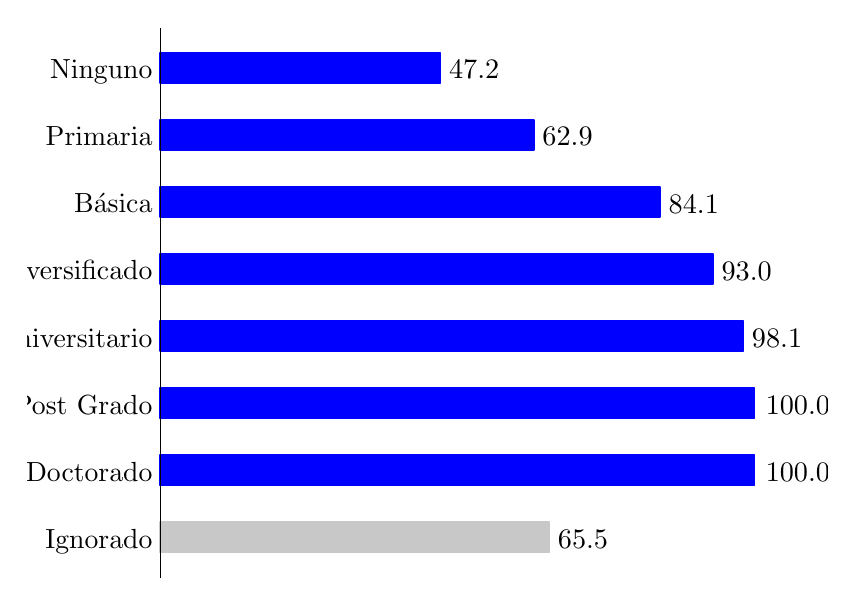
\begin{tikzpicture}[x=1pt,y=1pt]  % Created by tikzDevice version 0.10.1 on 2016-02-29 14:40:50
% !TEX encoding = UTF-8 Unicode
\definecolor{fillColor}{RGB}{255,255,255}
\path[use as bounding box,fill=fillColor,fill opacity=0.00] (0,0) rectangle (289.08,198.74);
\begin{scope}
\path[clip] (  0.00,  0.00) rectangle (289.08,198.74);

\path[] (  0.00,  0.00) rectangle (289.08,198.74);
\end{scope}
\begin{scope}
\path[clip] (  0.00,  0.00) rectangle (289.08,198.74);

\path[] ( 47.80,  0.00) rectangle (262.69,198.74);

\path[] ( 47.80, 14.54) --
	(262.69, 14.54);

\path[] ( 47.80, 38.78) --
	(262.69, 38.78);

\path[] ( 47.80, 63.02) --
	(262.69, 63.02);

\path[] ( 47.80, 87.25) --
	(262.69, 87.25);

\path[] ( 47.80,111.49) --
	(262.69,111.49);

\path[] ( 47.80,135.73) --
	(262.69,135.73);

\path[] ( 47.80,159.96) --
	(262.69,159.96);

\path[] ( 47.80,184.20) --
	(262.69,184.20);
\definecolor{drawColor}{RGB}{200,200,200}
\definecolor{fillColor}{RGB}{200,200,200}

\path[draw=drawColor,line width= 0.6pt,line join=round,fill=fillColor] ( 47.80,  9.09) rectangle (188.47, 20.00);
\definecolor{drawColor}{RGB}{0,0,255}
\definecolor{fillColor}{RGB}{0,0,255}

\path[draw=drawColor,line width= 0.6pt,line join=round,fill=fillColor] ( 47.80, 33.33) rectangle (262.69, 44.23);

\path[draw=drawColor,line width= 0.6pt,line join=round,fill=fillColor] ( 47.80, 57.56) rectangle (262.69, 68.47);

\path[draw=drawColor,line width= 0.6pt,line join=round,fill=fillColor] ( 47.80, 81.80) rectangle (258.60, 92.71);

\path[draw=drawColor,line width= 0.6pt,line join=round,fill=fillColor] ( 47.80,106.04) rectangle (247.60,116.94);

\path[draw=drawColor,line width= 0.6pt,line join=round,fill=fillColor] ( 47.80,130.27) rectangle (228.53,141.18);

\path[draw=drawColor,line width= 0.6pt,line join=round,fill=fillColor] ( 47.80,154.51) rectangle (182.89,165.42);

\path[draw=drawColor,line width= 0.6pt,line join=round,fill=fillColor] ( 47.80,178.75) rectangle (149.14,189.65);
\definecolor{drawColor}{RGB}{0,0,0}

\path[draw=drawColor,line width= 0.1pt,line join=round] ( 47.80,  0.00) -- ( 47.80,198.74);

\node[text=drawColor,anchor=base west,inner sep=0pt, outer sep=0pt, scale=  1.02] at (191.60, 10.57) {65.5};

\node[text=drawColor,anchor=base west,inner sep=0pt, outer sep=0pt, scale=  1.02] at (266.71, 34.81) {100.0};

\node[text=drawColor,anchor=base west,inner sep=0pt, outer sep=0pt, scale=  1.02] at (266.71, 59.04) {100.0};

\node[text=drawColor,anchor=base west,inner sep=0pt, outer sep=0pt, scale=  1.02] at (261.73, 83.28) {98.1};

\node[text=drawColor,anchor=base west,inner sep=0pt, outer sep=0pt, scale=  1.02] at (250.73,107.52) {93.0};

\node[text=drawColor,anchor=base west,inner sep=0pt, outer sep=0pt, scale=  1.02] at (231.65,131.76) {84.1};

\node[text=drawColor,anchor=base west,inner sep=0pt, outer sep=0pt, scale=  1.02] at (186.01,155.99) {62.9};

\node[text=drawColor,anchor=base west,inner sep=0pt, outer sep=0pt, scale=  1.02] at (152.27,180.23) {47.2};

\path[] ( 47.80,  0.00) rectangle (262.69,198.74);
\end{scope}
\begin{scope}
\path[clip] (  0.00,  0.00) rectangle (289.08,198.74);

\path[] ( 47.80,  0.00) --
	( 47.80,198.74);
\end{scope}
\begin{scope}
\path[clip] (  0.00,  0.00) rectangle (289.08,198.74);
\definecolor{drawColor}{RGB}{0,0,0}

\node[text=drawColor,anchor=base east,inner sep=0pt, outer sep=0pt, scale=  1.00] at ( 45.05, 10.63) {Ignorado};

\node[text=drawColor,anchor=base east,inner sep=0pt, outer sep=0pt, scale=  1.00] at ( 45.05, 34.87) {Doctorado};

\node[text=drawColor,anchor=base east,inner sep=0pt, outer sep=0pt, scale=  1.00] at ( 45.05, 59.11) {Post Grado};

\node[text=drawColor,anchor=base east,inner sep=0pt, outer sep=0pt, scale=  1.00] at ( 45.05, 83.34) {Universitario};

\node[text=drawColor,anchor=base east,inner sep=0pt, outer sep=0pt, scale=  1.00] at ( 45.05,107.58) {Diversificado};

\node[text=drawColor,anchor=base east,inner sep=0pt, outer sep=0pt, scale=  1.00] at ( 45.05,131.82) {Básica};

\node[text=drawColor,anchor=base east,inner sep=0pt, outer sep=0pt, scale=  1.00] at ( 45.05,156.06) {Primaria};

\node[text=drawColor,anchor=base east,inner sep=0pt, outer sep=0pt, scale=  1.00] at ( 45.05,180.29) {Ninguno};
\end{scope}
\begin{scope}
\path[clip] (  0.00,  0.00) rectangle (289.08,198.74);

\path[] ( 45.05, 14.54) --
	( 47.80, 14.54);

\path[] ( 45.05, 38.78) --
	( 47.80, 38.78);

\path[] ( 45.05, 63.02) --
	( 47.80, 63.02);

\path[] ( 45.05, 87.25) --
	( 47.80, 87.25);

\path[] ( 45.05,111.49) --
	( 47.80,111.49);

\path[] ( 45.05,135.73) --
	( 47.80,135.73);

\path[] ( 45.05,159.96) --
	( 47.80,159.96);

\path[] ( 45.05,184.20) --
	( 47.80,184.20);
\end{scope}
  \end{tikzpicture}}{Instituto Nacional de Estadística, de las Estadísticas Vitales 2014}

\cajita{Madres sin escolaridad que recibieron atención médica}{La tendencia de los nacimientos en madres sin educación que reciben atención médica ha sido ascendente.}{Proporción de nacimientos en madres sin educación, que recibieron atención médica}{República de Guatemala, serie histórica, en porcentaje}{\ \\[0mm]\begin{tikzpicture}[x=1pt,y=1pt]  % Created by tikzDevice version 0.10.1 on 2016-02-29 14:41:35
% !TEX encoding = UTF-8 Unicode
\definecolor{fillColor}{RGB}{255,255,255}
\path[use as bounding box,fill=fillColor,fill opacity=0.00] (0,0) rectangle (289.08,198.74);
\begin{scope}
\path[clip] (  0.00,  0.00) rectangle (289.08,198.74);

\path[] (  0.00,  0.00) rectangle (289.08,198.74);
\end{scope}
\begin{scope}
\path[clip] (  0.00,  0.00) rectangle (289.08,198.74);

\path[] ( -0.52, 15.61) rectangle (280.54,191.48);

\path[] (  0.00, 37.46) --
	(280.54, 37.46);

\path[] (  0.00, 72.10) --
	(280.54, 72.10);

\path[] (  0.00,106.74) --
	(280.54,106.74);

\path[] (  0.00,141.37) --
	(280.54,141.37);

\path[] (  0.00,176.01) --
	(280.54,176.01);

\path[] (  0.00, 20.14) --
	(280.54, 20.14);

\path[] (  0.00, 54.78) --
	(280.54, 54.78);

\path[] (  0.00, 89.42) --
	(280.54, 89.42);

\path[] (  0.00,124.05) --
	(280.54,124.05);

\path[] (  0.00,158.69) --
	(280.54,158.69);

\path[] ( 31.91, 15.61) --
	( 31.91,191.48);

\path[] ( 85.96, 15.61) --
	( 85.96,191.48);

\path[] (140.01, 15.61) --
	(140.01,191.48);

\path[] (194.06, 15.61) --
	(194.06,191.48);

\path[] (248.11, 15.61) --
	(248.11,191.48);
\definecolor{drawColor}{RGB}{0,0,255}

\path[draw=drawColor,line width= 1.7pt,line join=round] ( 31.91,138.26) --
	( 85.96,151.77) --
	(140.01,154.19) --
	(194.06,167.70) --
	(248.11,183.49);
\definecolor{drawColor}{RGB}{0,0,0}

\node[text=drawColor,anchor=base,inner sep=0pt, outer sep=0pt, scale=  1.02] at ( 31.91,126.34) {34.1};

\node[text=drawColor,anchor=base east,inner sep=0pt, outer sep=0pt, scale=  1.02] at ( 82.83,151.77) {38.0};

\node[text=drawColor,anchor=base east,inner sep=0pt, outer sep=0pt, scale=  1.02] at (136.88,154.19) {38.7};

\node[text=drawColor,anchor=base east,inner sep=0pt, outer sep=0pt, scale=  1.02] at (190.94,167.70) {42.6};

\node[text=drawColor,anchor=base,inner sep=0pt, outer sep=0pt, scale=  1.02] at (248.11,187.46) {47.2};

\path[draw=drawColor,line width= 0.1pt,line join=round] (  0.00, 23.61) -- (280.54, 23.61);

\path[] ( -0.52, 15.61) rectangle (280.54,191.48);
\end{scope}
\begin{scope}
\path[clip] (  0.00,  0.00) rectangle (289.08,198.74);

\path[] (  0.00, 15.61) --
	(280.54, 15.61);
\end{scope}
\begin{scope}
\path[clip] (  0.00,  0.00) rectangle (289.08,198.74);

\path[] ( 31.91, 12.86) --
	( 31.91, 15.61);

\path[] ( 85.96, 12.86) --
	( 85.96, 15.61);

\path[] (140.01, 12.86) --
	(140.01, 15.61);

\path[] (194.06, 12.86) --
	(194.06, 15.61);

\path[] (248.11, 12.86) --
	(248.11, 15.61);
\end{scope}
\begin{scope}
\path[clip] (  0.00,  0.00) rectangle (289.08,198.74);
\definecolor{drawColor}{RGB}{0,0,0}

\node[text=drawColor,anchor=base,inner sep=0pt, outer sep=0pt, scale=  1.00] at ( 31.91,  2.85) {2010};

\node[text=drawColor,anchor=base,inner sep=0pt, outer sep=0pt, scale=  1.00] at ( 85.96,  2.85) {2011};

\node[text=drawColor,anchor=base,inner sep=0pt, outer sep=0pt, scale=  1.00] at (140.01,  2.85) {2012};

\node[text=drawColor,anchor=base,inner sep=0pt, outer sep=0pt, scale=  1.00] at (194.06,  2.85) {2013};

\node[text=drawColor,anchor=base,inner sep=0pt, outer sep=0pt, scale=  1.00] at (248.11,  2.85) {2014};
\end{scope}
  \end{tikzpicture}}{Instituto Nacional de Estadística, de las Estadísticas Vitales 2014}


\cajota{Madres sin escolaridad que recibieron atención médica\newline en los departamentos}{Los departamentos con menor proporción de nacimientos que recibieron atención médica, en madres sin educación fueron: Huehuetenango (20.4\%), San Marcos (29.4\%), Quiché (25.3\%), Totonicapán (30.5\%) y Sololá (35.0\%).}{Proporción de nacimientos de madres sin escolaridad que recibieron atención médica}{Departamental, 2014, en porcentaje}{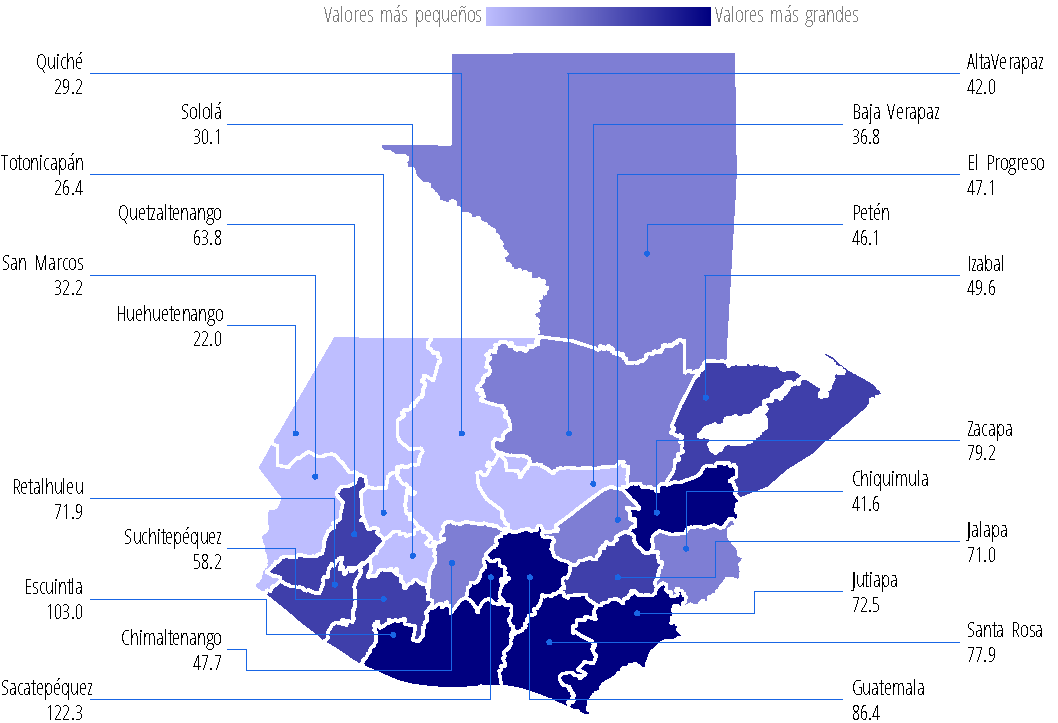
\includegraphics[width=52\cuadri]{graficas/vitales/1_11.pdf}}{Instituto Nacional de Estadística, de las Estadísticas Vitales 2014}


\cajita{Nacimientos ocurridos en centro médico, según escolaridad la madre}{\footnote{Incluye los nacimientos ocurridos en: hospital privado, hospital público, centro de salud e IGSS} Los nacimientos ocurridos en el 2014, el 97.1\% de las madres con educación superior recibió atención en un centro médico, por otro lado, solo el 43.4\% de las madres sin educación tuvo atención médica en este tipo de centro.}{Proporción de nacimientos que ocurrieron en centro médico, según el nivel de escolaridad de la madre}{República de Guatemala, 2014, en porcentaje}{\ \\[0mm]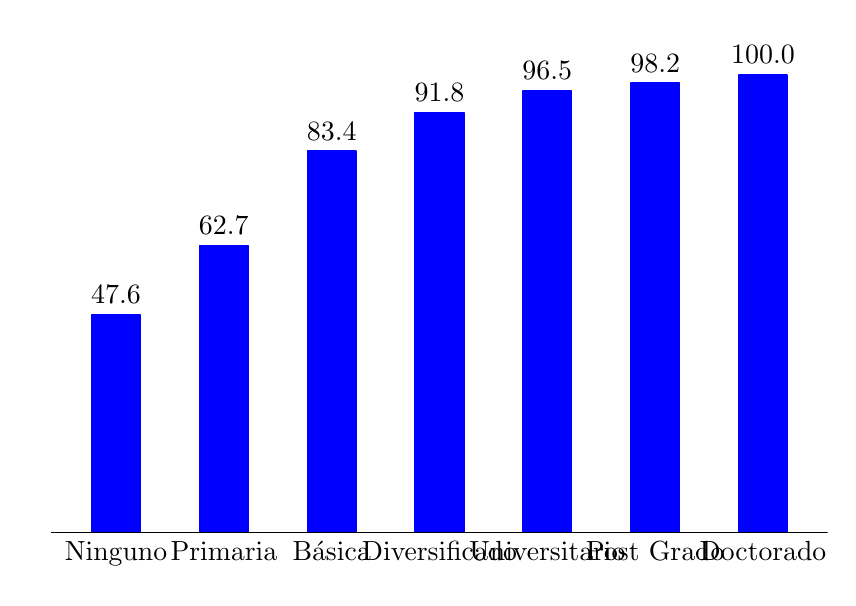
\begin{tikzpicture}[x=1pt,y=1pt]  % Created by tikzDevice version 0.8.1 on 2015-12-10 16:21:53
% !TEX encoding = UTF-8 Unicode
\definecolor{fillColor}{RGB}{255,255,255}
\path[use as bounding box,fill=fillColor,fill opacity=0.00] (0,0) rectangle (289.08,198.74);
\begin{scope}
\path[clip] (  0.00,  0.00) rectangle (289.08,198.74);

\path[] (  0.00,  0.00) rectangle (289.08,198.74);
\end{scope}
\begin{scope}
\path[clip] (  0.00,  0.00) rectangle (289.08,198.74);

\path[] (  8.54, 16.35) rectangle (289.08,181.67);

\path[] ( 31.91, 16.35) --
	( 31.91,181.67);

\path[] ( 70.88, 16.35) --
	( 70.88,181.67);

\path[] (109.84, 16.35) --
	(109.84,181.67);

\path[] (148.81, 16.35) --
	(148.81,181.67);

\path[] (187.77, 16.35) --
	(187.77,181.67);

\path[] (226.74, 16.35) --
	(226.74,181.67);

\path[] (265.70, 16.35) --
	(265.70,181.67);
\definecolor{drawColor}{RGB}{0,0,255}
\definecolor{fillColor}{RGB}{0,0,255}

\path[draw=drawColor,line width= 0.6pt,line join=round,fill=fillColor] ( 23.15, 16.35) rectangle ( 40.68, 95.06);

\path[draw=drawColor,line width= 0.6pt,line join=round,fill=fillColor] ( 62.11, 16.35) rectangle ( 79.65,120.04);

\path[draw=drawColor,line width= 0.6pt,line join=round,fill=fillColor] (101.08, 16.35) rectangle (118.61,154.19);

\path[draw=drawColor,line width= 0.6pt,line join=round,fill=fillColor] (140.04, 16.35) rectangle (157.57,168.08);

\path[draw=drawColor,line width= 0.6pt,line join=round,fill=fillColor] (179.01, 16.35) rectangle (196.54,175.89);

\path[draw=drawColor,line width= 0.6pt,line join=round,fill=fillColor] (217.97, 16.35) rectangle (235.50,178.72);

\path[draw=drawColor,line width= 0.6pt,line join=round,fill=fillColor] (256.93, 16.35) rectangle (274.47,181.67);
\definecolor{drawColor}{RGB}{0,0,0}

\path[draw=drawColor,line width= 0.1pt,line join=round] (  8.54, 16.35) -- (289.08, 16.35);

\node[text=drawColor,anchor=base,inner sep=0pt, outer sep=0pt, scale=  1.01] at ( 31.91, 99.02) {47.6};

\node[text=drawColor,anchor=base,inner sep=0pt, outer sep=0pt, scale=  1.01] at ( 70.88,124.00) {62.7};

\node[text=drawColor,anchor=base,inner sep=0pt, outer sep=0pt, scale=  1.01] at (109.84,158.15) {83.4};

\node[text=drawColor,anchor=base,inner sep=0pt, outer sep=0pt, scale=  1.01] at (148.81,172.04) {91.8};

\node[text=drawColor,anchor=base,inner sep=0pt, outer sep=0pt, scale=  1.01] at (187.77,179.85) {96.5};

\node[text=drawColor,anchor=base,inner sep=0pt, outer sep=0pt, scale=  1.01] at (226.74,182.68) {98.2};

\node[text=drawColor,anchor=base,inner sep=0pt, outer sep=0pt, scale=  1.01] at (265.70,185.63) {100.0};

\path[] (  8.54, 16.35) rectangle (289.08,181.67);
\end{scope}
\begin{scope}
\path[clip] (  0.00,  0.00) rectangle (289.08,198.74);

\path[] (  8.54, 16.35) --
	(  8.54,181.67);
\end{scope}
\begin{scope}
\path[clip] (  0.00,  0.00) rectangle (289.08,198.74);

\path[] (  8.54, 16.35) --
	(289.08, 16.35);
\end{scope}
\begin{scope}
\path[clip] (  0.00,  0.00) rectangle (289.08,198.74);

\path[] ( 31.91, 12.08) --
	( 31.91, 16.35);

\path[] ( 70.88, 12.08) --
	( 70.88, 16.35);

\path[] (109.84, 12.08) --
	(109.84, 16.35);

\path[] (148.81, 12.08) --
	(148.81, 16.35);

\path[] (187.77, 12.08) --
	(187.77, 16.35);

\path[] (226.74, 12.08) --
	(226.74, 16.35);

\path[] (265.70, 12.08) --
	(265.70, 16.35);
\end{scope}
\begin{scope}
\path[clip] (  0.00,  0.00) rectangle (289.08,198.74);
\definecolor{drawColor}{RGB}{0,0,0}

\node[text=drawColor,anchor=base,inner sep=0pt, outer sep=0pt, scale=  1.00] at ( 31.91,  6.04) {Ninguno};

\node[text=drawColor,anchor=base,inner sep=0pt, outer sep=0pt, scale=  1.00] at ( 70.88,  6.04) {Primaria};

\node[text=drawColor,anchor=base,inner sep=0pt, outer sep=0pt, scale=  1.00] at (109.84,  6.04) {Básica};

\node[text=drawColor,anchor=base,inner sep=0pt, outer sep=0pt, scale=  1.00] at (148.81,  6.04) {Diversificado};

\node[text=drawColor,anchor=base,inner sep=0pt, outer sep=0pt, scale=  1.00] at (187.77,  6.04) {Universitario};

\node[text=drawColor,anchor=base,inner sep=0pt, outer sep=0pt, scale=  1.00] at (226.74,  6.04) {Post Grado};

\node[text=drawColor,anchor=base,inner sep=0pt, outer sep=0pt, scale=  1.00] at (265.70,  6.04) {Doctorado};
\end{scope}
  \end{tikzpicture}}{Instituto Nacional de Estadística, de las Estadísticas Vitales 2014}

\cajita{Nacimientos ocurridos en centro médico, madres sin escolaridad}{La tendencia de los nacimientos en madres sin educación que reciben atención en un centro médico ha sido ascendente.}{Proporción de nacimientos en madres sin escolaridad, que ocurrieron en centros de atención médica}{República de Guatemala, serie histórica, en porcentaje}{\ \\[0mm]\begin{tikzpicture}[x=1pt,y=1pt]  % Created by tikzDevice version 0.10.1 on 2016-02-29 14:42:24
% !TEX encoding = UTF-8 Unicode
\definecolor{fillColor}{RGB}{255,255,255}
\path[use as bounding box,fill=fillColor,fill opacity=0.00] (0,0) rectangle (289.08,198.74);
\begin{scope}
\path[clip] (  0.00,  0.00) rectangle (289.08,198.74);

\path[] (  0.00,  0.00) rectangle (289.08,198.74);
\end{scope}
\begin{scope}
\path[clip] (  0.00,  0.00) rectangle (289.08,198.74);

\path[] ( -0.52, 15.61) rectangle (280.54,191.48);

\path[] (  0.00, 40.40) --
	(280.54, 40.40);

\path[] (  0.00, 73.98) --
	(280.54, 73.98);

\path[] (  0.00,107.56) --
	(280.54,107.56);

\path[] (  0.00,141.14) --
	(280.54,141.14);

\path[] (  0.00,174.72) --
	(280.54,174.72);

\path[] (  0.00, 23.61) --
	(280.54, 23.61);

\path[] (  0.00, 57.19) --
	(280.54, 57.19);

\path[] (  0.00, 90.77) --
	(280.54, 90.77);

\path[] (  0.00,124.35) --
	(280.54,124.35);

\path[] (  0.00,157.93) --
	(280.54,157.93);

\path[] ( 31.91, 15.61) --
	( 31.91,191.48);

\path[] ( 85.96, 15.61) --
	( 85.96,191.48);

\path[] (140.01, 15.61) --
	(140.01,191.48);

\path[] (194.06, 15.61) --
	(194.06,191.48);

\path[] (248.11, 15.61) --
	(248.11,191.48);
\definecolor{drawColor}{RGB}{0,0,255}

\path[draw=drawColor,line width= 1.7pt,line join=round] ( 31.91,138.45) --
	( 85.96,151.88) --
	(140.01,153.90) --
	(194.06,169.34) --
	(248.11,183.49);
\definecolor{drawColor}{RGB}{0,0,0}

\node[text=drawColor,anchor=base,inner sep=0pt, outer sep=0pt, scale=  1.02] at ( 31.91,126.54) {34.2};

\node[text=drawColor,anchor=base east,inner sep=0pt, outer sep=0pt, scale=  1.02] at ( 82.83,151.88) {38.2};

\node[text=drawColor,anchor=base east,inner sep=0pt, outer sep=0pt, scale=  1.02] at (136.88,153.90) {38.8};

\node[text=drawColor,anchor=base east,inner sep=0pt, outer sep=0pt, scale=  1.02] at (190.94,169.34) {43.4};

\node[text=drawColor,anchor=base,inner sep=0pt, outer sep=0pt, scale=  1.02] at (248.11,187.46) {47.6};

\path[draw=drawColor,line width= 0.1pt,line join=round] (  0.00, 23.61) -- (280.54, 23.61);

\path[] ( -0.52, 15.61) rectangle (280.54,191.48);
\end{scope}
\begin{scope}
\path[clip] (  0.00,  0.00) rectangle (289.08,198.74);

\path[] (  0.00, 15.61) --
	(280.54, 15.61);
\end{scope}
\begin{scope}
\path[clip] (  0.00,  0.00) rectangle (289.08,198.74);

\path[] ( 31.91, 12.86) --
	( 31.91, 15.61);

\path[] ( 85.96, 12.86) --
	( 85.96, 15.61);

\path[] (140.01, 12.86) --
	(140.01, 15.61);

\path[] (194.06, 12.86) --
	(194.06, 15.61);

\path[] (248.11, 12.86) --
	(248.11, 15.61);
\end{scope}
\begin{scope}
\path[clip] (  0.00,  0.00) rectangle (289.08,198.74);
\definecolor{drawColor}{RGB}{0,0,0}

\node[text=drawColor,anchor=base,inner sep=0pt, outer sep=0pt, scale=  1.00] at ( 31.91,  2.85) {2010};

\node[text=drawColor,anchor=base,inner sep=0pt, outer sep=0pt, scale=  1.00] at ( 85.96,  2.85) {2011};

\node[text=drawColor,anchor=base,inner sep=0pt, outer sep=0pt, scale=  1.00] at (140.01,  2.85) {2012};

\node[text=drawColor,anchor=base,inner sep=0pt, outer sep=0pt, scale=  1.00] at (194.06,  2.85) {2013};

\node[text=drawColor,anchor=base,inner sep=0pt, outer sep=0pt, scale=  1.00] at (248.11,  2.85) {2014};
\end{scope}
  \end{tikzpicture}}{Instituto Nacional de Estadística, de las Estadísticas Vitales 2014}

\cajota{Madres sin escolaridad que recibieron atención médica\newline en los departamentos}{Los departamentos con menor proporción de nacimientos en madres sin educación  que recibieron atención en un centro médico, fueron: Huehuetenango (20.8\%), San Marcos (29.2\%), Quiché (25.4\%), Totonicapán (30.3\%) y Sololá (34.1\%).}{Nacimientos en madres sin educación que recibieron atención médica}{Departamental,2014, en porcentaje}{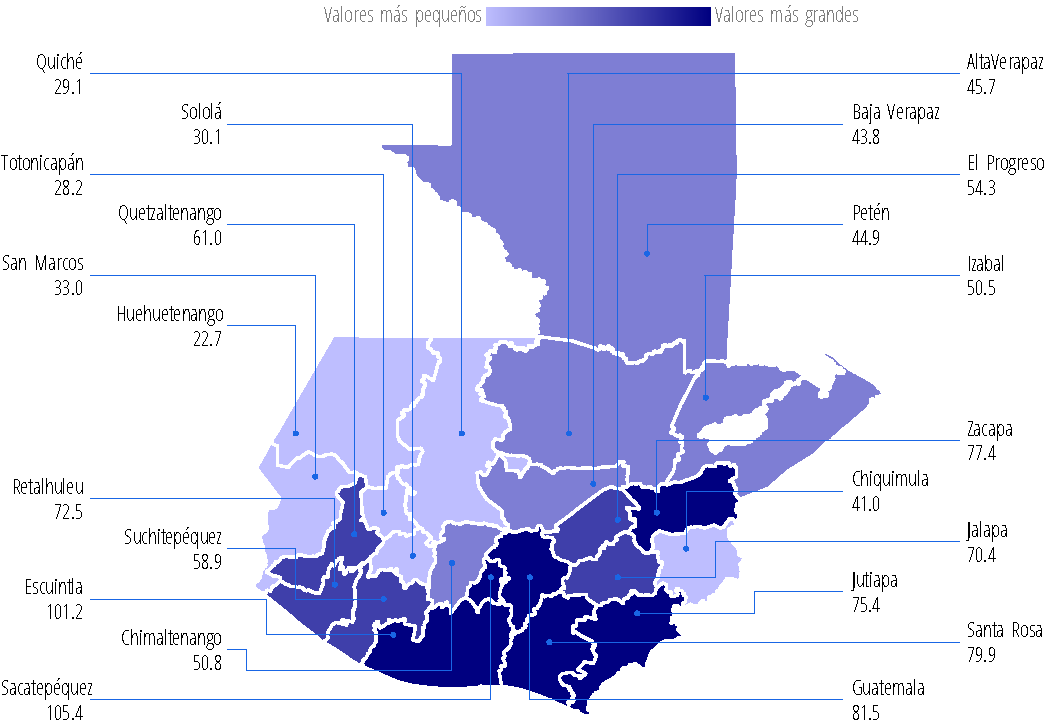
\includegraphics[width=52\cuadri]{graficas/vitales/1_14.pdf}}{Instituto Nacional de Estadística, de las Estadísticas Vitales 2014}
